\documentclass[conference]{IEEEtran}
\IEEEoverridecommandlockouts
\usepackage{ragged2e}
\usepackage{graphicx}
\usepackage{float}
\usepackage{adjustbox}
\usepackage[utf8]{inputenc}
\usepackage{amsmath}
\usepackage{booktabs}
\usepackage{siunitx}
\usepackage{hyperref}
\usepackage{tikz}
\usetikzlibrary{shapes.geometric, arrows, calc}

\tikzstyle{startstop} = [rectangle, rounded corners, minimum width=3cm,
  minimum height=1cm, text centered, draw=black, fill=red!30]
\tikzstyle{process}   = [rectangle, minimum width=3cm, minimum height=1cm,
  text centered, draw=black, fill=orange!30]
\tikzstyle{decision}  = [diamond, minimum width=3cm, minimum height=1cm,
  text centered, draw=black, fill=green!30]
\tikzstyle{arrow}     = [thick,->,>=stealth]

\usepackage[margin=1in]{geometry}
\sloppy

% ── Title and author ──────────────────────────────────────────
\title{Spatial Statistics Methods for the Analysis of
  Infectious Disease \textit{Clusters} in Latin America}

\author{
  \IEEEauthorblockN{Jhon Cristhian Gonzales Quispe}
  \IEEEauthorblockA{
    \textit{Faculty of Statistical and Computer Engineering}\\
    \textit{Universidad Nacional del Altiplano}\\
    Puno, Per\'u\\
    j.gonzales@est.unap.edu.pe
  }
}

\begin{document}
\maketitle
% ── Abstract ────────────────────────────────────────────────
\begin{abstract}
The detection of infectious disease clusters through spatial
statistics methods is a central strategy in modern
epidemiological surveillance. However, no systematic synthesis
exists that characterizes these methods within the Latin American
context. This article presents a systematic review following the
PRISMA~2020 guidelines, with searches conducted in Scopus and
IEEE~Xplore for the period 2015--2025. After an automated
screening process and manual review, 76~articles were selected
that explicitly employ spatial methods in infectious disease
studies conducted in Latin America. The results show that the
global Moran's~I index and LISA analysis are the most frequent
methods (31.6\% each), followed by SaTScan (23.7\%) and
Getis-Ord~Gi* (13.2\%). Brazil accounts for 88.2\% of
publications. The most studied diseases are dengue and
arboviruses (23.7\%), leishmaniasis (19.7\%), tuberculosis
(15.8\%), and COVID-19 (14.5\%). A methodological gap is
identified in the use of hierarchical Bayesian
spatio-temporal models, which are underrepresented in the
region despite their well-recognized robustness. These findings
guide the geospatial research agenda in public health for
Latin America.
\end{abstract}

\begin{IEEEkeywords}
spatial statistics, infectious diseases, Latin America,
cluster detection, systematic review,
PRISMA~2020, geospatial epidemiology, Moran's index,
SaTScan, Bayesian models
\end{IEEEkeywords}

% ════════════════════════════════════════════════════════════
\section{Introduction}
% ════════════════════════════════════════════════════════════

In the contemporary epidemiological context, infectious
diseases continue to represent one of the greatest threats to
public health and global socioeconomic stability. Their
management demands not only clinical responses, but also the
development of advanced analytical tools that allow their
spread to be anticipated, modeled, and mitigated
\cite{Delmelle2023}. In recent decades, the integration of
geospatial analysis into epidemiology has transformed the
understanding of transmission dynamics, making it possible to
observe how environmental and social factors interact within
a given territory \cite{Lin2022}.

Spatial statistics has established itself as a fundamental
pillar for identifying non-random patterns in the distribution
of diseases. Its applications span four major areas:
visualization, detection of global clustering, identification
of \textit{hotspots}, and risk factor modeling with adjustment
for spatial heterogeneity \cite{Lin2022}. Advanced
methodologies such as Bayesian spatio-temporal models have
demonstrated high effectiveness in the early detection of
transmission clusters, as evidenced during the COVID-19
health crisis in 2020 \cite{Zhu2022, Chen2022}. These
approaches provide health systems with an empirical basis for
the optimal allocation of resources and the design of
targeted intervention policies \cite{LevinRector2024}.

Latin America faces particular challenges due to its
geographic heterogeneity, socioeconomic gaps, and the
persistence of emerging and re-emerging diseases. Brazil, for
example, recorded in 2024 its largest historical dengue
epidemic with more than six million cases \cite{Sena2025}.
Colombia has accumulated more than 319,567 leishmaniasis cases
over four decades, with hotspots concentrated in Amazonian and
Pacific regions \cite{Leishmaniasis2025}. In Peru, geospatial
studies in Lima have demonstrated that routine surveillance
data are sufficient to identify high-incidence tuberculosis
areas at the neighborhood scale \cite{Brooks2022}.

Despite these advances, no systematic synthesis yet exists
that comprehensively compares the spatial methodological
approaches used in the Latin American context over the last
decade. This gap makes it difficult to identify the most
robust methods, the most studied diseases, and the recurrent
limitations in the literature \cite{Delmelle2023,
Habereder2025}.

With the aim of providing a clear and structured overview,
this article presents a systematic review of the scientific
literature produced between 2015 and 2025. The main spatial
statistics methods used for the analysis of infectious disease
\textit{clusters} in the Latin American context are examined
and compared, discussing their scope, limitations, and
relevance in modern epidemiological surveillance.

% ════════════════════════════════════════════════════════════
\section{Methodology}
% ════════════════════════════════════════════════════════════

\subsection{Study Design}

A systematic literature review was conducted following the
guidelines established by PRISMA~2020 (\textit{Preferred
Reporting Items for Systematic Reviews and Meta-Analyses})
\cite{Page2021}. The review aimed to identify and analyze the
spatial statistics methods used in studies on infectious
diseases conducted in Latin America during the period
2015--2025.

\subsection{Research Question}

The research question was formulated using the PECO framework:

\begin{itemize}
  \item \textbf{P (Population):} populations in Latin America
    and the Caribbean affected by infectious diseases.
  \item \textbf{E (Exposure):} application of spatial
    statistics methods in epidemiological analysis.
  \item \textbf{C (Comparison):} comparison among different
    spatial methods used for the detection and analysis of
    epidemiological patterns.
  \item \textbf{O (Outcome):} identification of clusters,
    spatial patterns, and factors associated with the
    geographic distribution of infectious diseases.
\end{itemize}

From this framework the following question was formulated:
\textit{What are the main spatial statistics methods used for
the analysis of infectious disease clusters in Latin America,
and what are their most frequent applications during the
period 2015--2025?}

\subsection{Information Sources}

The bibliographic search was conducted in the Scopus and
IEEE~Xplore databases, due to their broad coverage of indexed
scientific publications in the areas of public health,
epidemiology, statistics, informatics, and geospatial
analysis. Retrieved records were exported in RIS format,
including title, authors, abstract, keywords, year of
publication, journal, and source.

\subsection{Search Strategy}

The search was carried out using terms related to spatial
statistics, epidemiology, and infectious diseases. The general
search equation used was:

\begin{quote}
\small
\texttt{
("spatial statistics" OR "spatial analysis" OR\\
"geostatistics" OR "hotspot analysis" OR\\
"SaTScan" OR "Moran index" OR "LISA" OR\\
"Kriging" OR "GWR" OR "DBSCAN")\\
AND\\
("infectious disease" OR "epidemiology" OR\\
"dengue" OR "malaria" OR "tuberculosis" OR\\
"COVID-19" OR "leishmaniasis")\\
AND\\
("Latin America" OR "South America" OR\\
"Peru" OR "Brazil" OR "Colombia" OR\\
"Mexico" OR "Bolivia" OR "Ecuador")\\
AND PUBYEAR > 2014
}
\end{quote}

The search was limited to publications in English and Spanish
published between 2015 and 2025.

\subsection{Eligibility Criteria}

\subsubsection{Inclusion Criteria}
\begin{itemize}
  \item Scientific articles published between 2015 and 2025.
  \item Studies that explicitly employ spatial statistics
    methods.
  \item Research related to infectious diseases.
  \item Studies conducted in Latin American and Caribbean
    countries.
  \item Publications indexed in Scopus or IEEE~Xplore.
\end{itemize}

\subsubsection{Exclusion Criteria}
\begin{itemize}
  \item Studies conducted outside the Latin American context.
  \item Research without application of spatial methods.
  \item Review articles, editorials, letters to the editor,
    or conference abstracts.
  \item Duplicate records.
  \item Studies with insufficient information to determine
    eligibility.
\end{itemize}

\subsection{Data Retrieval and Preparation}

The bibliographic records obtained from Scopus and
IEEE~Xplore were exported in RIS format and integrated into
a single database. Subsequently, a metadata normalization
process was carried out to unify field names, correct
inconsistencies, and eliminate duplicate records through
comparison of normalized titles.

\subsection{Tools Used}

Various support tools were used for the development of the
review. Mendeley was used for the management and verification
of bibliographic references. RStudio was used for reading RIS
files, integrating records, removing duplicates, applying
automatic selection criteria, and generating preliminary
descriptive statistics. The libraries \texttt{revtools},
\texttt{dplyr}, \texttt{stringr}, \texttt{purrr},
\texttt{ggplot2}, and \texttt{writexl} were used for
automated information processing.

\subsection{Automated Screening Process}

Due to the large number of retrieved records, an automated
procedure was developed in RStudio to carry out a first
screening phase. The algorithm evaluated the content of
titles, abstracts, and keywords using specialized
dictionaries built from three categories: (1)~spatial
statistics methods, (2)~infectious diseases, and
(3)~Latin American countries and regions.

Each record received a relevance score based on compliance
with these criteria and was classified into one of three
categories:

\begin{itemize}
  \item \textbf{INCLUDE:} studies that simultaneously meet
    the thematic, methodological, and geographic criteria.
  \item \textbf{UNCERTAIN:} potentially relevant studies
    requiring additional manual review.
  \item \textbf{EXCLUDE:} studies that do not meet the
    established criteria.
\end{itemize}

\subsection{Selection Process}

The selection of studies was carried out in two phases. The
first phase corresponded to the automated screening described
above. The second phase consisted of the manual review of
titles, abstracts, and full texts of studies classified as
potentially eligible, in order to confirm their definitive
inclusion in the systematic review. After this stage, the
sample was composed of \textbf{76~articles}.

\subsection{Methodological Quality Assessment}

The methodological quality of the selected studies was
assessed using the CASP (\textit{Critical Appraisal Skills
Programme}) tool, which classifies studies according to their
quality level and risk of bias.

\subsection{PRISMA~2020 Flowchart}

The complete process of identification, screening,
eligibility assessment, and inclusion is summarized in
Figure~\ref{fig:prisma}.

\begin{figure}[t]
\centering
\resizebox{\columnwidth}{!}{%
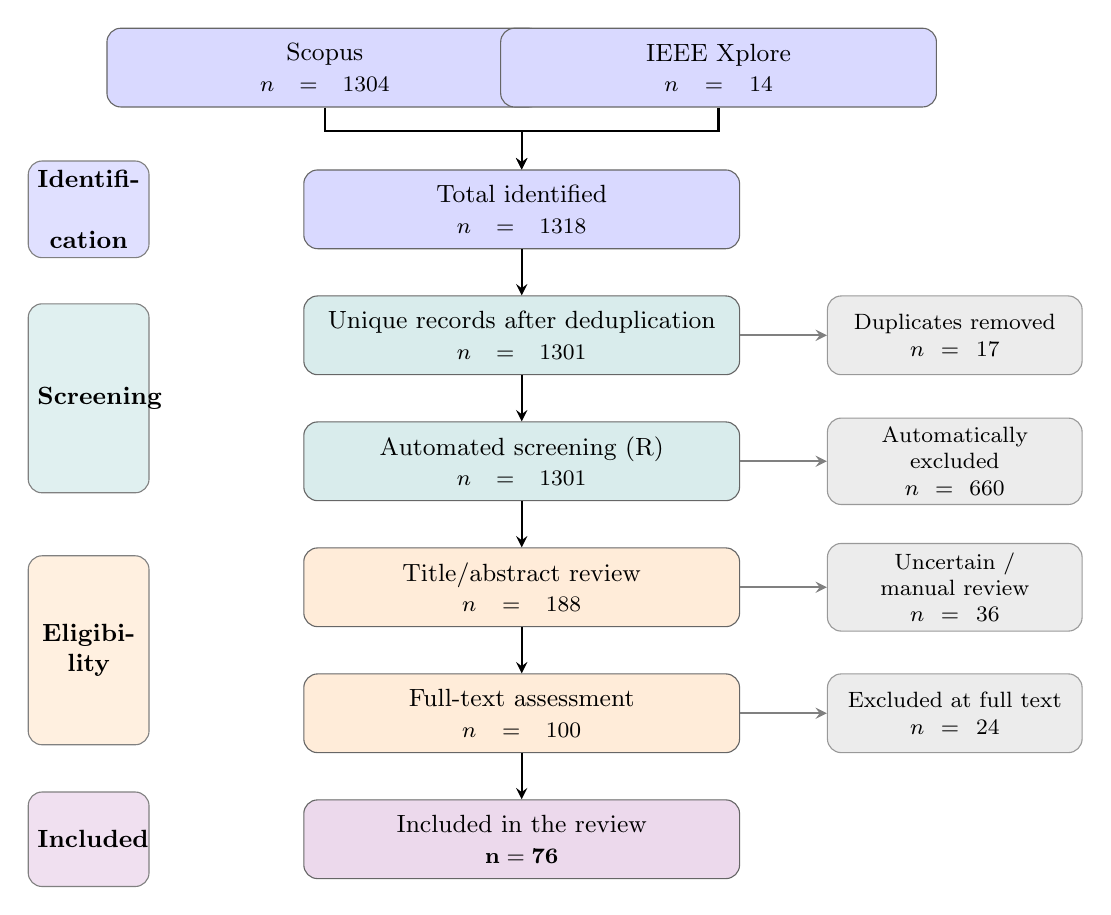
\begin{tikzpicture}

\tikzset{
  caja/.style={rectangle, rounded corners=5pt,
    minimum width=5.5cm, minimum height=1cm,
    text centered, draw=black!60,
    font=\small, text width=5.3cm},
  excl/.style={rectangle, rounded corners=5pt,
    minimum width=3.2cm, minimum height=1cm,
    text centered, draw=black!40,
    font=\footnotesize, text width=3cm, fill=gray!15},
  fase/.style={rectangle, rounded corners=5pt,
    minimum width=1.5cm,
    text centered, draw=black!50,
    font=\small\bfseries, text width=1.3cm},
  arrow/.style={->, >=stealth, thick}
}

% ---- CENTRAL NODES ----
\node (scopus)   [caja, fill=blue!15]   at (-2.5, 0)
  {Scopus\\{\footnotesize $n = 1304$}};
\node (ieee)     [caja, fill=blue!15]   at ( 2.5, 0)
  {IEEE Xplore\\{\footnotesize $n = 14$}};
\node (total)    [caja, fill=blue!15]   at (   0,-1.8)
  {Total identified\\{\footnotesize $n = 1318$}};
\node (unicos)   [caja, fill=teal!15]   at (   0,-3.4)
  {Unique records after deduplication\\{\footnotesize $n = 1301$}};
\node (cribado)  [caja, fill=teal!15]   at (   0,-5.0)
  {Automated screening (R)\\{\footnotesize $n = 1301$}};
\node (titulo)   [caja, fill=orange!15] at (   0,-6.6)
  {Title/abstract review\\{\footnotesize $n = 188$}};
\node (completo) [caja, fill=orange!15] at (   0,-8.2)
  {Full-text assessment\\{\footnotesize $n = 100$}};
\node (incluidos)[caja, fill=violet!15] at (   0,-9.8)
  {Included in the review\\{\footnotesize $\mathbf{n = 76}$}};

% ---- EXCLUDED (right) ----
\node (dup)      [excl] at (5.5,-3.4)
  {Duplicates removed\\{\footnotesize $n = 17$}};
\node (excl660)  [excl] at (5.5,-5.0)
  {Automatically excluded\\{\footnotesize $n = 660$}};
\node (inciertos)[excl] at (5.5,-6.6)
  {Uncertain / manual review\\{\footnotesize $n = 36$}};
\node (excltc)   [excl] at (5.5,-8.2)
  {Excluded at full text\\{\footnotesize $n = 24$}};

% ---- PHASE LABELS (left) ----
\node (fid)[fase, fill=blue!12,   minimum height=1.2cm]
  at (-5.5,-1.8){Identifi-\\cation};
\node (fsc)[fase, fill=teal!12,   minimum height=2.4cm]
  at (-5.5,-4.2){Screening};
\node (fel)[fase, fill=orange!12, minimum height=2.4cm]
  at (-5.5,-7.4){Eligibi-\\lity};
\node (fin)[fase, fill=violet!12, minimum height=1.2cm]
  at (-5.5,-9.8){Included};

% ---- MAIN ARROWS ----
\draw[arrow] (scopus.south)  -- ++(0,-0.3) -| (total.north);
\draw[arrow] (ieee.south)    -- ++(0,-0.3) -| (total.north);
\draw[arrow] (total)    -- (unicos);
\draw[arrow] (unicos)   -- (cribado);
\draw[arrow] (cribado)  -- (titulo);
\draw[arrow] (titulo)   -- (completo);
\draw[arrow] (completo) -- (incluidos);

% ---- ARROWS TO EXCLUDED ----
\draw[arrow, gray] (unicos.east)   -- (dup.west);
\draw[arrow, gray] (cribado.east)  -- (excl660.west);
\draw[arrow, gray] (titulo.east)   -- (inciertos.west);
\draw[arrow, gray] (completo.east) -- (excltc.west);

\end{tikzpicture}
}
\caption{PRISMA~2020 flow diagram --- final sample $n = 76$.}
\label{fig:prisma}
\end{figure}

% ════════════════════════════════════════════════════════════
\section{Results}
% ════════════════════════════════════════════════════════════

\subsection{Selection Process Results}

The search strategy applied in Scopus and IEEE~Xplore
initially identified 1,318 bibliographic records. Of these,
1,304 came from Scopus and 14 from IEEE~Xplore. After removing
17 duplicate records through comparison of normalized titles,
a consolidated database of 1,301 unique articles was obtained.

The automated screening process automatically discarded 660
articles and flagged 36 as uncertain for manual review. The
605 preliminarily included articles were subjected to
successive prioritization stages that reduced the set to 188
articles. Of these, 100 high-relevance studies were selected
for the full-text assessment phase. After detailed reading,
24 articles that did not fully meet the inclusion criteria
were excluded, yielding a final sample of
\textbf{76 articles}
\cite{FloresSacoto2025, Miranda2024, DeLima2025, Souza2023,
Konczycki2025, Silva2024, Tavares2024, Lalangui2024,
deLima2024, Matos2025, Silva2025, Santos2024,
AlmeidadeSouza2024, BirchenallJimenez2024, Perotto2025,
DaudtLemos2025, Paz2023, Gomes2023, dosSantos2024,
Saavedra2025, Lopes2025, Pungartnik2025, deFreitas2024,
MedeirosSilva2025, Gomes2023b, CharlesLeija2024, Veloso2025,
Bermudi2025, Freitas2024, DeLima2025, Damasceno2025,
deMelo2024, daSilva2024, Biazussi2025, Silveira2024,
Rocha2025, VieiraDuarte2024, Leandro2024, deSousa2024,
Alves2021, Guo2020, Alves2022, DzulManzanilla2021,
Silva2023, Berra2020, Siqueira2021, doCarmo2020,
daSilva2022, Wangdi2022, Adegboye2021, Pereira2021,
Pereira2021b, SoaresSantana2021,
doSocorroCarvalhoMiranda2022, GaytcanCamarillo2021,
daSilva2023, Schultes2021, Miranda2021, FcalixRocha2023,
Nina2023, Costa2021, DeOliveira2021, Huang2021,
Skalinski2022, Braga2021, Braz2021, Coutinho2022,
daSilvaSoeiro2022, Medeiros2023, Echenique2021,
Leandro2022, CortesEscamilla2022, deMelo2023, Ueno2021,
Castro2021, Queiroz2021}.

\begin{table}[t]
\centering
\caption{Summary of the PRISMA~2020 selection process}
\label{tab:cribado}
\begin{tabular}{lr}
\toprule
Stage & Count \\
\midrule
Records identified in Scopus           & 1,304 \\
Records identified in IEEE~Xplore      & 14    \\
Total identified                        & 1,318 \\
Duplicates removed                      & 17    \\
Unique records                          & 1,301 \\
Automatically excluded                  & 660   \\
Uncertain for manual review             & 36    \\
Preliminarily included                  & 605   \\
\midrule
\textbf{Prioritized articles}           & \textbf{188} \\
\textbf{Selected for full-text review}  & \textbf{100} \\
\textbf{Excluded at full text}          & \textbf{24}  \\
\textbf{Final included sample}          & \textbf{76}  \\
\bottomrule
\end{tabular}
\end{table}

\subsection{Temporal Distribution}

The 76 included articles were published between 2020 and
2025 (Figure~\ref{fig:anios}). A sustained increase in
scientific output in the area is observed, with a marked
rise starting in 2021. The years 2021, 2024, and 2025
account for the largest share of publications, with 19, 18,
and 17 articles respectively, reflecting the surge in
geospatial epidemiological studies in Latin America during
and after the COVID-19 pandemic.

\begin{figure}[t]
\centering
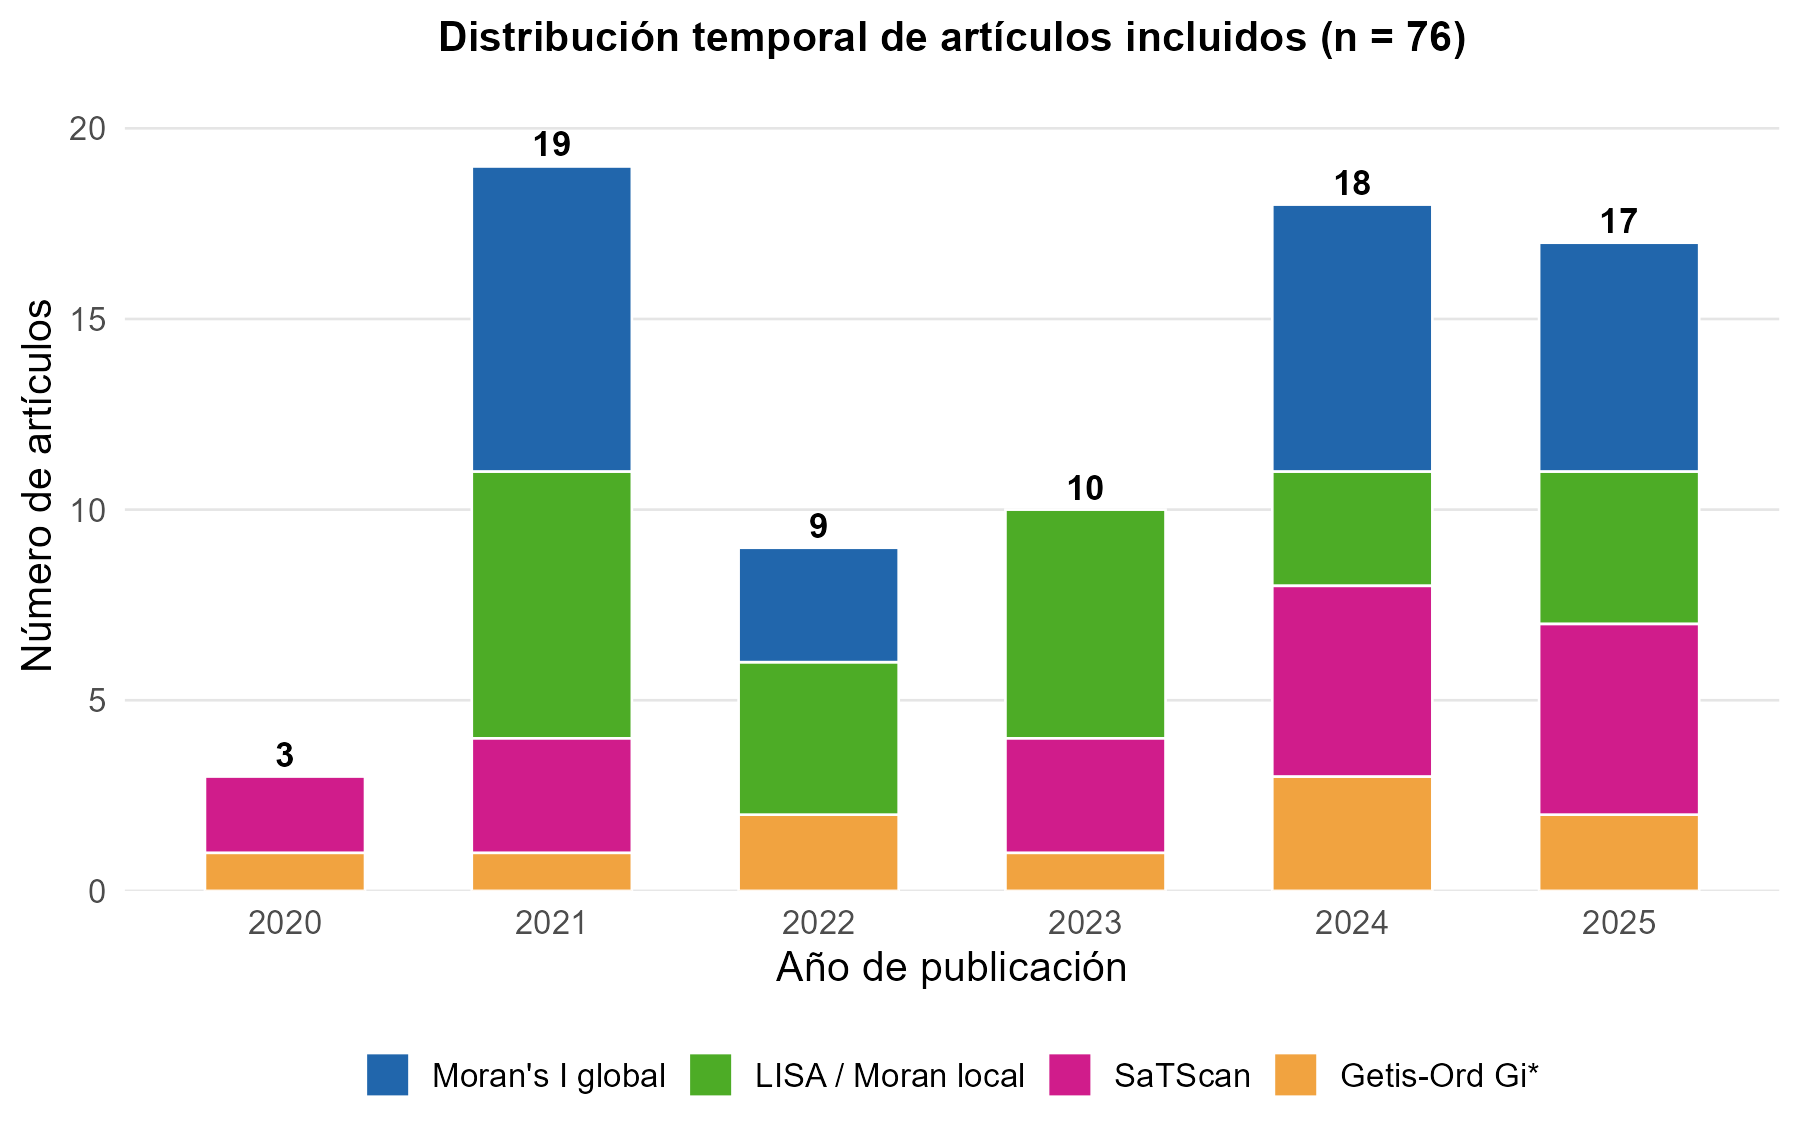
\includegraphics[width=0.48\textwidth]{fig1_anios.png}
\caption{Temporal distribution of included articles
  ($n = 76$).}
\label{fig:anios}
\end{figure}

\subsection{Distribution by Country}

Brazil widely dominates the regional scientific output in
this field, accounting for 67 of the 76 included articles
(88.2\%), followed at a distance by Mexico (3; 3.9\%),
Ecuador (2; 2.6\%), and Colombia (2; 2.6\%)
(Figure~\ref{fig:paises}). This concentration reflects both
the magnitude of the infectious disease burden in Brazil and
the established tradition of its academic institutions and
epidemiological surveillance systems in the use of geospatial
tools.

\begin{figure}[t]
\centering
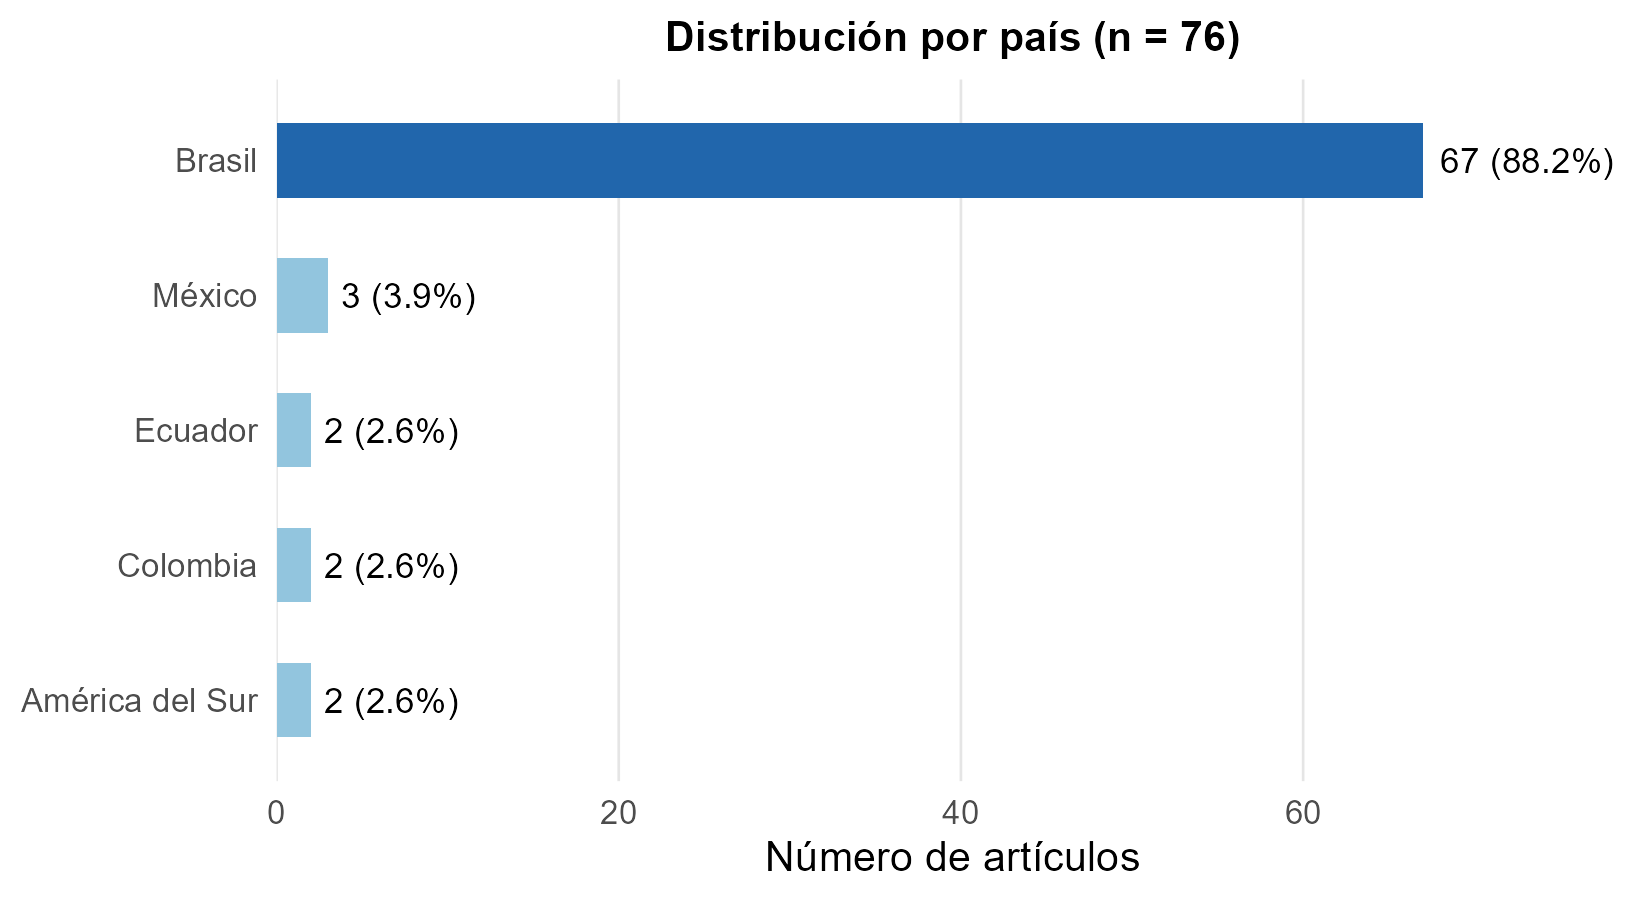
\includegraphics[width=0.48\textwidth]{fig2_paises.png}
\caption{Distribution by country ($n = 76$).}
\label{fig:paises}
\end{figure}

\subsection{Distribution by Disease}

The infectious diseases most studied through spatial
statistics methods were dengue and arboviruses combined
(18; 23.7\%), leishmaniasis (15; 19.7\%), tuberculosis
(12; 15.8\%), and COVID-19 (11; 14.5\%)
(Figure~\ref{fig:enfermedades}). A smaller proportion of
studies was identified on leprosy (5), malaria (4), Chagas
disease (2), schistosomiasis (2), and other infectious
diseases.

\begin{figure}[t]
\centering
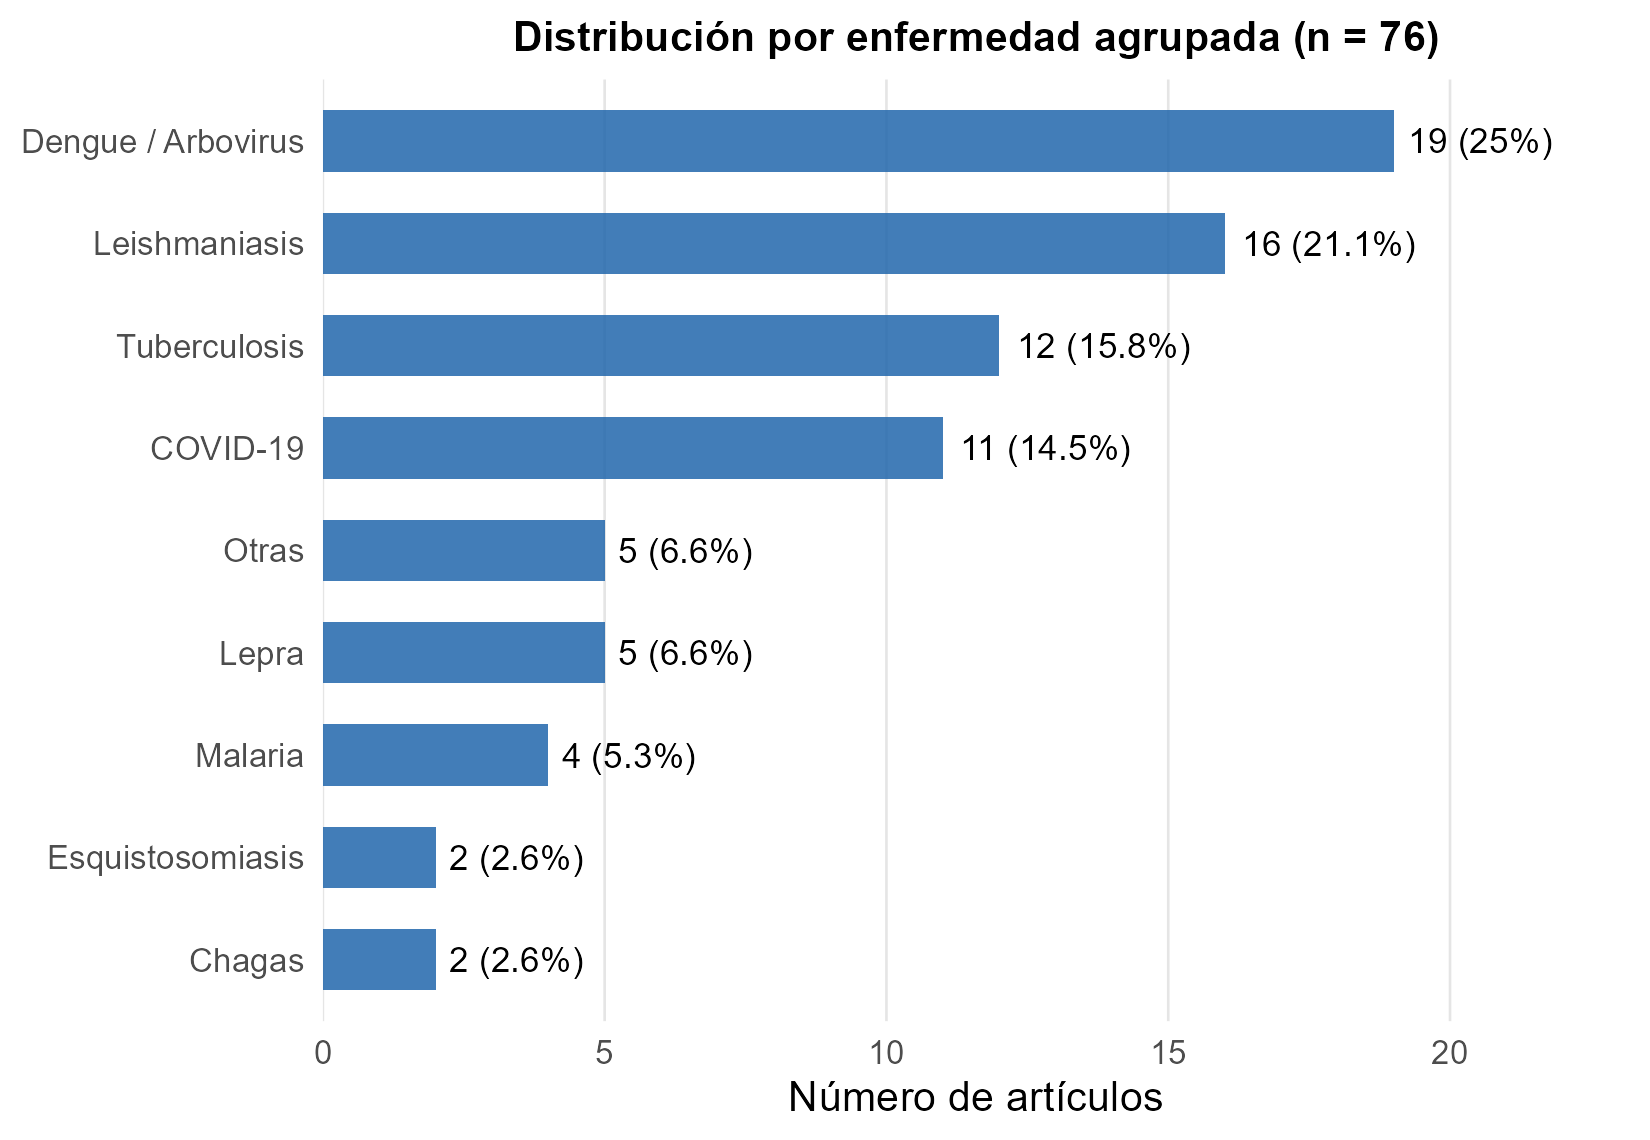
\includegraphics[width=0.48\textwidth]{fig3_enfermedades.png}
\caption{Distribution by grouped disease ($n = 76$).}
\label{fig:enfermedades}
\end{figure}

\subsection{Spatial Methods Identified}

The four spatial statistics methods identified in the final
sample show a relatively balanced distribution between global
and local autocorrelation techniques
(Figure~\ref{fig:metodos}). The global Moran's~I index and
LISA (\textit{Local Indicators of Spatial Association})
analysis are the most frequent, with 24 articles each
(31.6\% respectively), followed by SaTScan with 18 articles
(23.7\%) and Getis-Ord~Gi* with 10 articles (13.2\%).

Studies based on global Moran's~I
\cite{FloresSacoto2025, Miranda2024, Lalangui2024, deLima2024,
Santos2024, DaudtLemos2025, Lopes2025, MedeirosSilva2025,
CharlesLeija2024, DeLima2025, daSilva2024, Rocha2025,
Leandro2024, Alves2022, Siqueira2021, Adegboye2021,
Pereira2021, Pereira2021b, doSocorroCarvalhoMiranda2022,
Miranda2021, Huang2021, Braz2021, CortesEscamilla2022,
Queiroz2021}
focus predominantly on the detection of spatial
autocorrelation at national or state scale. Those employing
LISA / local Moran
\cite{DeLima2025, Konczycki2025, Matos2025,
BirchenallJimenez2024, Perotto2025, Gomes2023, Gomes2023b,
VieiraDuarte2024, deSousa2024, Silva2023, SoaresSantana2021,
GaytcanCamarillo2021, daSilva2023, Schultes2021, Nina2023,
Costa2021, DeOliveira2021, Skalinski2022, Braga2021,
Coutinho2022, daSilvaSoeiro2022, Medeiros2023, Leandro2022,
Castro2021}
add the identification of local clusters (high-high,
low-low quadrants, etc.). SaTScan
\cite{Souza2023, Silva2025, AlmeidadeSouza2024, Paz2023,
Saavedra2025, deFreitas2024, Veloso2025, Bermudi2025,
Freitas2024, deMelo2024, Biazussi2025, Silveira2024,
Alves2021, Berra2020, doCarmo2020, Echenique2021,
deMelo2023, Ueno2021}
enables the detection of spatio-temporal clusters with
statistical significance. Getis-Ord~Gi*
\cite{Silva2024, Tavares2024, dosSantos2024, Pungartnik2025,
Damasceno2025, Guo2020, DzulManzanilla2021, daSilva2022,
Wangdi2022, FcalixRocha2023}
is used to identify local incidence \textit{hotspots} and
\textit{coldspots}.

\begin{figure}[t]
\centering
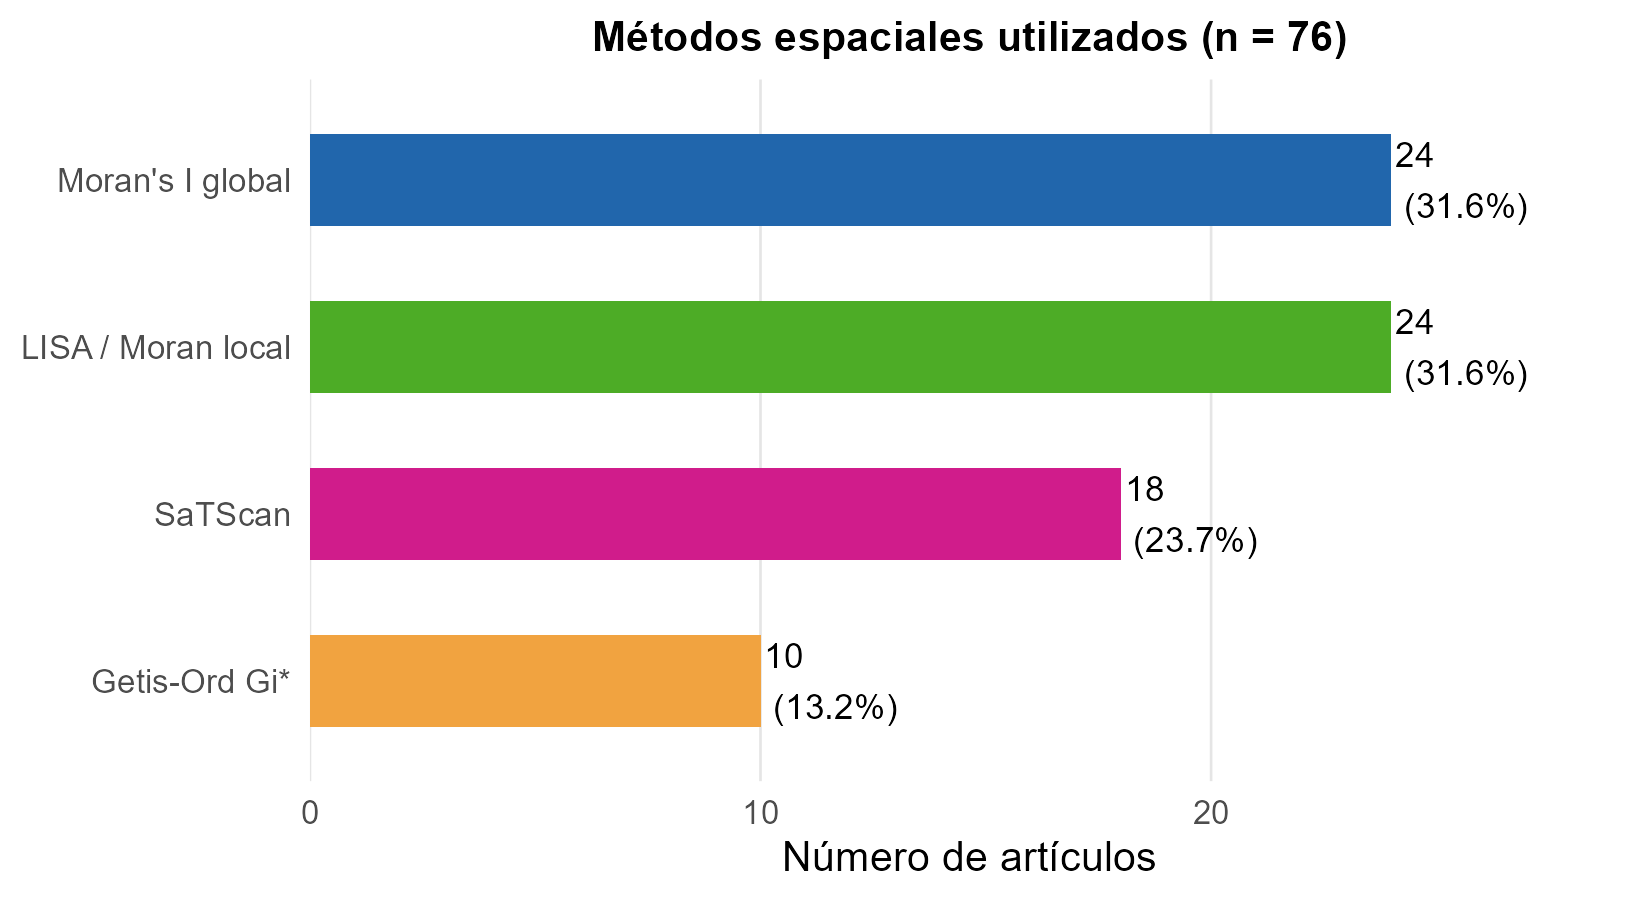
\includegraphics[width=0.48\textwidth]{fig4_metodos.png}
\caption{Spatial methods used ($n = 76$).}
\label{fig:metodos}
\end{figure}

\subsection{Relationship Between Methods and Diseases}

Figure~\ref{fig:heatmap} presents the heat map of the
frequency of method--disease combinations. Leishmaniasis is
studied primarily through global Moran's~I and LISA, while
tuberculosis shows the most diversified use of all four
methods. SaTScan concentrates its application on dengue and
tuberculosis. Getis-Ord~Gi* appears more frequently in
studies of tuberculosis and leishmaniasis.

\begin{figure}[t]
\centering
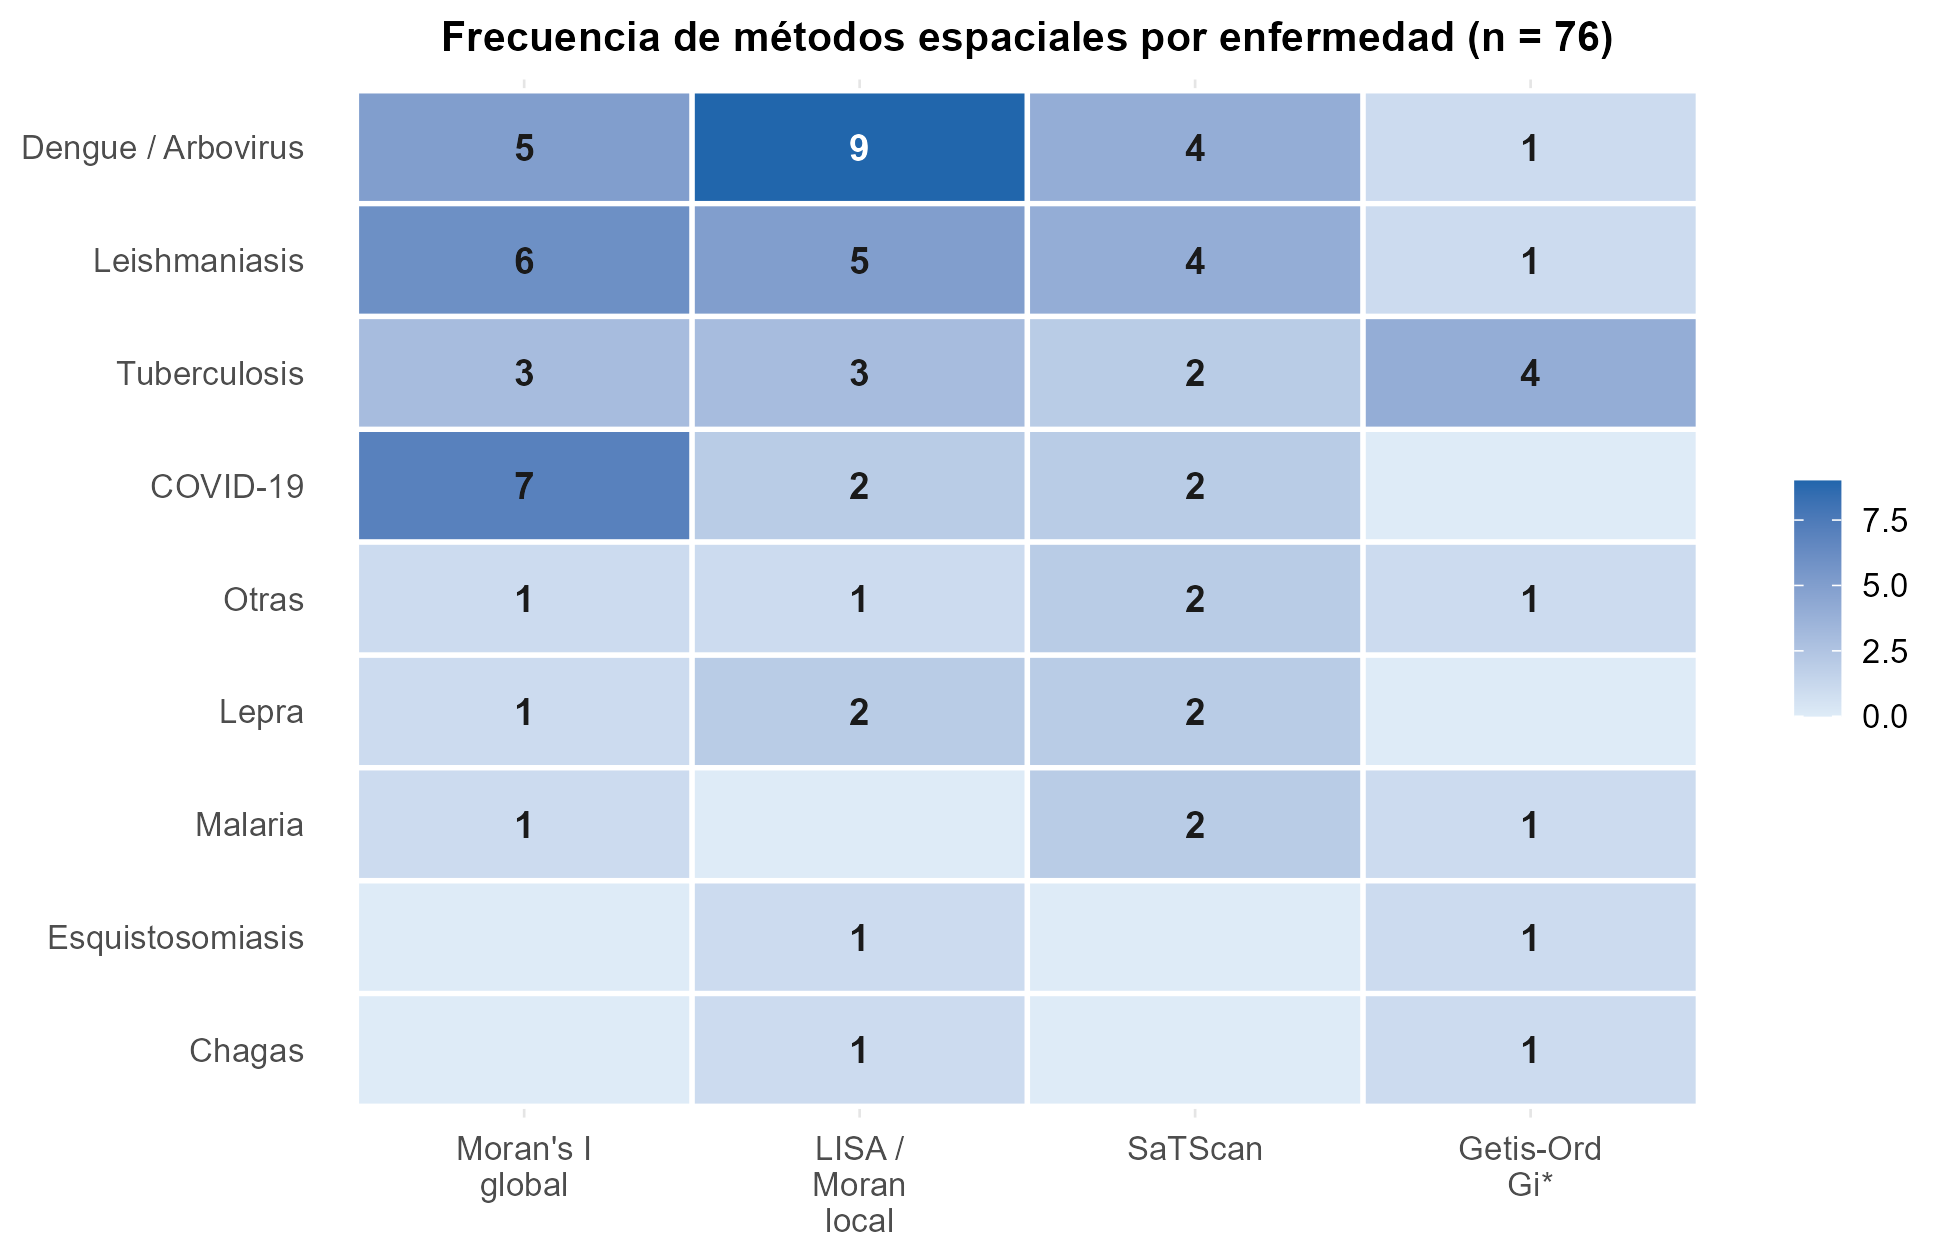
\includegraphics[width=0.48\textwidth]{fig5_heatmap.png}
\caption{Frequency of spatial methods by disease ($n = 76$).}
\label{fig:heatmap}
\end{figure}

% ════════════════════════════════════════════════════════════
\section{Discussion}
% ════════════════════════════════════════════════════════════

The results of this systematic review confirm that spatial
statistics has established itself as an indispensable tool
for the surveillance and analysis of infectious diseases in
Latin America during the period 2015--2025. The concentration
of studies in Brazil, the predominance of dengue and
leishmaniasis, and the preference for global and local
autocorrelation methods reflect both the regional
epidemiological burden and the institutional capacities of
each country to produce geospatial research.

\subsection{Brazil's Dominance in Regional Scientific Output}

The overwhelming proportion of studies from Brazil (88.2\%)
responds to well-documented structural factors. The country
has robust and publicly accessible epidemiological
surveillance systems, such as DATASUS, which facilitate the
retrieval of georeferenced data at the municipal scale
\cite{Souza2023}. Likewise, the high burden of neglected
tropical diseases, the ecological diversity of the Amazonian
territory, and the institutional resources of federal and
state universities explain this concentration
\cite{Miranda2024, DeLima2025}. This finding is consistent
with previous reviews noting that Latin American production
in geospatial epidemiology originates primarily in Brazil,
Colombia, and Mexico \cite{Delmelle2023}.

The scarce representation of countries such as Peru, Bolivia,
Paraguay, and much of Central America constitutes an
important limitation of the available literature, given that
many of these territories harbor endemic foci of
leishmaniasis, malaria, and tuberculosis without the
analytical coverage that their public health needs would
demand \cite{Habereder2025}.

\subsection{Spatial Methods: Trends and Applications}

The spatial autocorrelation methods, global Moran's~I and
LISA, are the most used in the analyzed sample (31.6\% each).
This prevalence reflects their straightforward implementation
in platforms such as GeoDa, R, and QGIS, as well as their
direct interpretability for public health decision-makers.
The global Moran's~I index provides a synthetic measure of
the non-random spatial distribution of a disease, while its
local complement---LISA---enables the identification of
specific municipalities or regions that form significant
clusters of high or low incidence \cite{Lin2022}.

SaTScan (23.7\%) differs from the above by incorporating the
temporal dimension, allowing the detection of clusters that
emerge or intensify during specific periods. This feature
makes it especially valuable for the analysis of diseases
with marked seasonal dynamics, such as dengue and
leptospirosis, or for evaluating the impact of public health
interventions \cite{Souza2023, Bermudi2025}. Getis-Ord~Gi*
(13.2\%) complements the others by identifying geographic
\textit{hotspots} of high local incidence with statistical
significance, being particularly useful in studies at the
municipal or neighborhood scale where internal heterogeneity
is high \cite{Tavares2024}.

It is worth noting that no study in the final sample
exclusively employed hierarchical Bayesian spatio-temporal
models, despite the international literature recognizing them
as the most suitable for modeling uncertainty in small areas
with low counts \cite{Zhu2022, Chen2022}. This
methodological gap represents a development opportunity for
Latin American epidemiological research, especially for the
analysis of re-emerging diseases and new events of public
health interest \cite{NIRAULA2026100961}.

\subsection{Most Studied Diseases}

Dengue and associated arboviruses account for the largest
proportion of studies (23.7\%), consistent with the historic
epidemic recorded in Brazil in 2024 and the endemic
situation in the region \cite{Sena2025}. The identified
studies demonstrate that spatial methods allow not only
mapping the distribution of cases, but also linking
transmission patterns with socio-environmental variables
such as vegetation cover, temperature, and drinking water
coverage \cite{Siqueira2021, DzulManzanilla2021}.

Leishmaniasis (19.7\%) ranks second, reflecting its endemic
nature in northern and northeastern Brazil, Colombia, and
Peru \cite{Miranda2024, Leishmaniasis2025}. The reviewed
studies predominantly use Moran's~I and LISA to identify
clusters in Amazonian and Pacific regions with high vector
exposure \cite{Konczycki2025, deSousa2024}.

Tuberculosis (15.8\%) appears as the disease with the
greatest methodological diversity in its geospatial analysis:
studies were identified using all four analyzed methods,
including SaTScan for the detection of spatio-temporal
clusters linked to the COVID-19 pandemic and the disruption
of control programs \cite{Souza2023, Perotto2025}. This
finding confirms that tuberculosis remains a sensitive
indicator of territorial social inequities and a productive
field for geospatial research.

\subsection{Limitations of the Review}

This review presents limitations that should be considered
when interpreting its results. First, the search was
restricted to two databases, which may have excluded relevant
studies published in regional repositories or in Portuguese
without indexing in Scopus. Second, the classification of
spatial methods was based primarily on information declared
in titles and abstracts, which may have underestimated the
presence of complementary approaches described only in the
methods sections of the articles. Finally, the geographic
concentration of the sample in Brazil limits the
generalizability of the findings to the Latin American
region as a whole.

% ════════════════════════════════════════════════════════════
\section{Conclusions}
% ════════════════════════════════════════════════════════════

This systematic review demonstrates that spatial statistics
methods have established themselves as indispensable tools
for the epidemiological surveillance of infectious diseases
in Latin America during the period 2015--2025. The analysis
of the 76~included articles allows the following conclusions
to be drawn.

First, the global Moran's~I index and LISA analysis are the
most widely used methods in the region (31.6\% each),
reflecting their accessibility in platforms such as GeoDa,
R, and QGIS, as well as their direct interpretability for
public health decision-makers. SaTScan stands out for
incorporating the temporal dimension, making it the
preferred tool for diseases with marked seasonal dynamics
such as dengue, while Getis-Ord~Gi* is particularly useful
for identifying local \textit{hotspots} at the municipal
scale.

Second, Brazil concentrates the largest regional scientific
output (88.2\%), supported by robust publicly accessible
surveillance systems such as DATASUS and a high burden of
tropical diseases. This concentration contrasts with the
scarce representation of countries such as Peru, Bolivia,
and much of Central America, where endemic foci of
leishmaniasis, malaria, and tuberculosis persist without
geospatial analytical coverage proportional to their disease
burden.

Third, dengue and arboviruses (23.7\%), leishmaniasis
(19.7\%), and tuberculosis (15.8\%) are the diseases most
studied through these methods, consistent with the
epidemiological burden of the region. The COVID-19 pandemic
also accelerated the development and application of
spatio-temporal models, demonstrating the value of these
approaches for decision-making in public health emergencies.

Finally, a significant methodological gap is identified:
hierarchical Bayesian spatio-temporal models, internationally
recognized as the most appropriate for modeling uncertainty
in small areas with low counts, are underrepresented in the
Latin American literature. Bridging this gap, together with
expanding the geographic coverage of studies toward countries
with less tradition in geospatial research, constitutes the
main pending agenda for spatial epidemiology in the region.

In summary, the systematic integration of spatial statistics
into epidemiological surveillance programs in Latin America
represents a key strategy for the early detection of
outbreaks, the prioritization of resources, and the design
of targeted interventions. Strengthening these analytical
capacities, especially in countries with greater health
vulnerability, is essential to prevent and mitigate the
impact of future public health emergencies.

% ════════════════════════════════════════════════════════════
\bibliographystyle{IEEEtran}
\bibliography{referencias}
% ════════════════════════════════════════════════════════════

\end{document}
